\section{Support Vector Machine}
\label{mainsec:svm}
\textit{Manuel Dudda, Benjamin Weißer}

Im Jahr 1958 veröffentlichte der Psycholge und Informatiker Frank Rosenblatt sein entwickeltes Konzept des Perzeptrons \cite{rosenblatt58a}. 
Die Idee entstammt der Neurobiologie und simuliert die Funktionsweise eines menschlichen Gehirns. 
Perzeptronen sind vereinfachte künstliche neuronale Netze, bestehend aus mehreren künstlichen Neuronen, die ein formales Modell einer Nervenzelle beschreiben. 
In der Grundversion besteht ein Perzeptron aus einem einzigen Neuron. 
Es verarbeitet einen Eingabevektor zu einer Ausgabe. 
Anhand eines Schwellwertes wird entschieden, ob das Neuron "{}feuert"{} oder nicht. 
Bei der Verarbeitung des Eingabevektors wird für jede Komponente eine Gewichtung berücksichtigt, sodass die Ausgabe auf gewisse Eingaben eingestellt werden kann. 
Mehrlagige Perzeptronen (MLP) sind in der Lage, Eingabevektoren in Ausgabevektoren umzuwandeln. 

\begin{figure}[htbp] \centering
    \subfigure[Pezeptron mit einem Neuron]{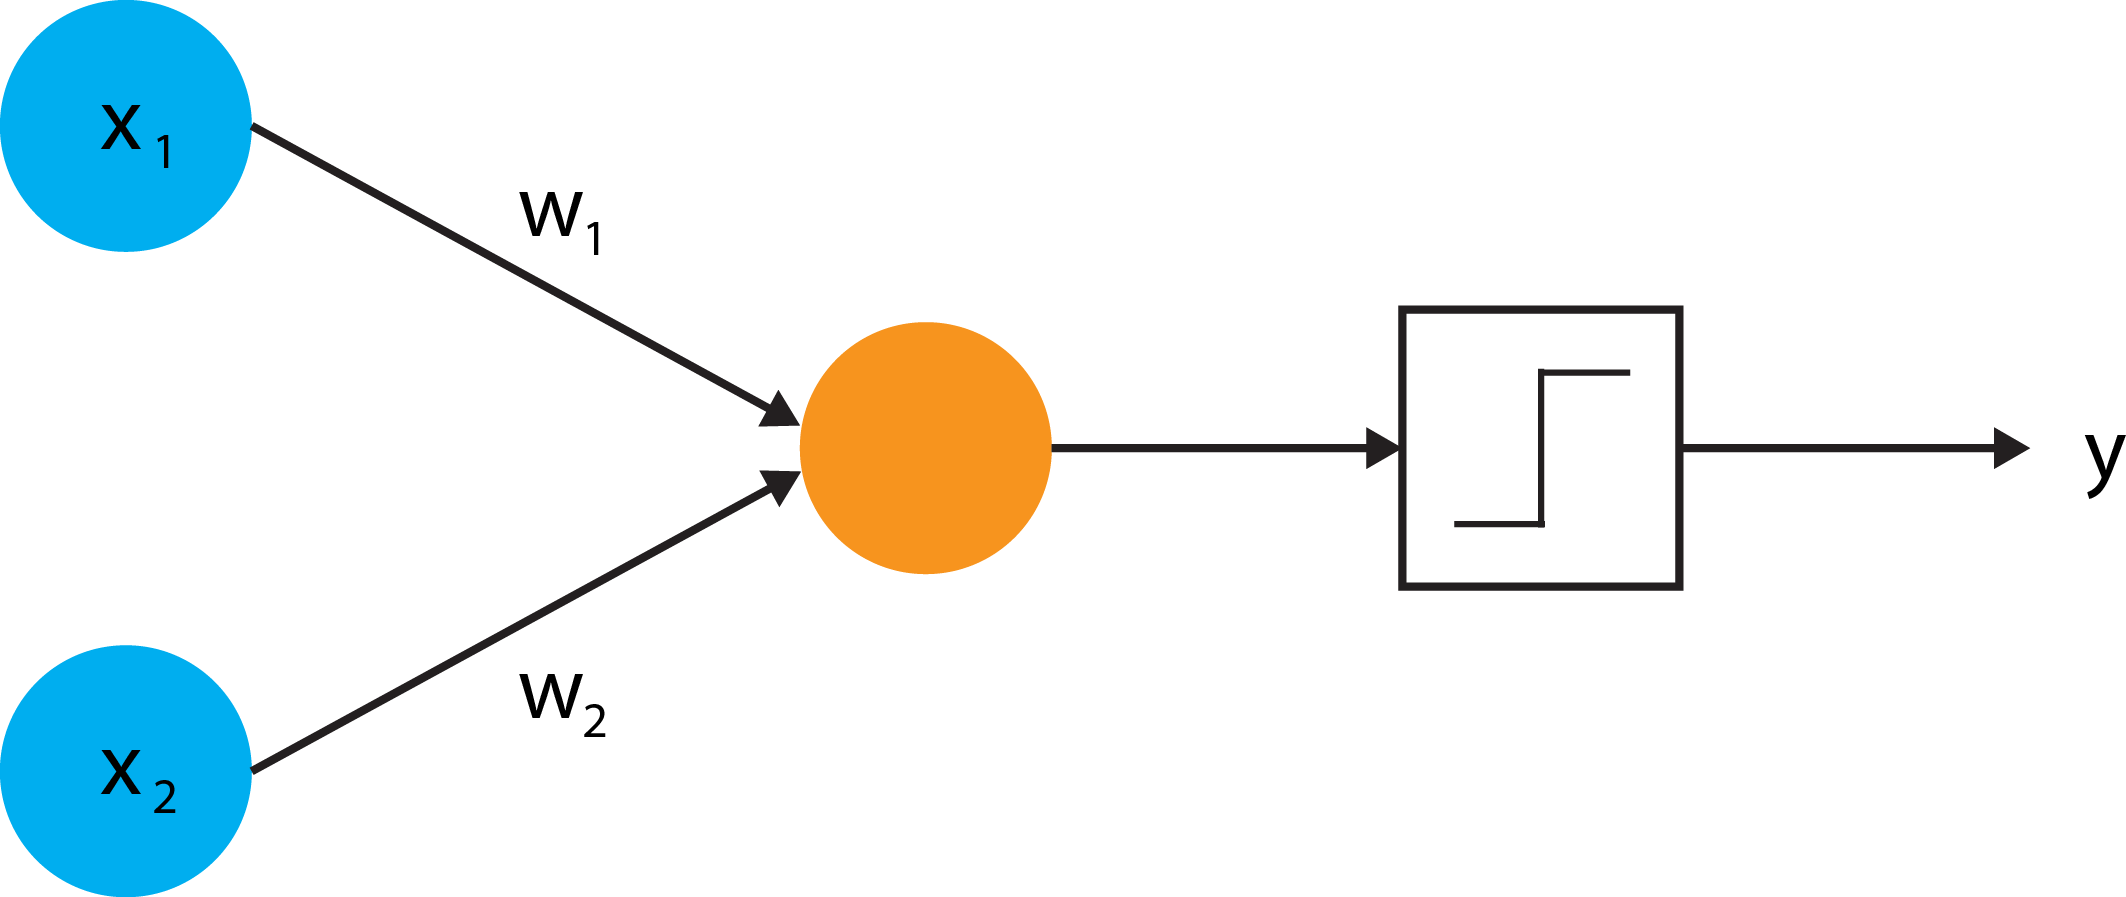
\includegraphics[width=0.22\textwidth]{svm/svm_perceptron.png}}
    \subfigure[Klassentrennung im Koordinatensystem]{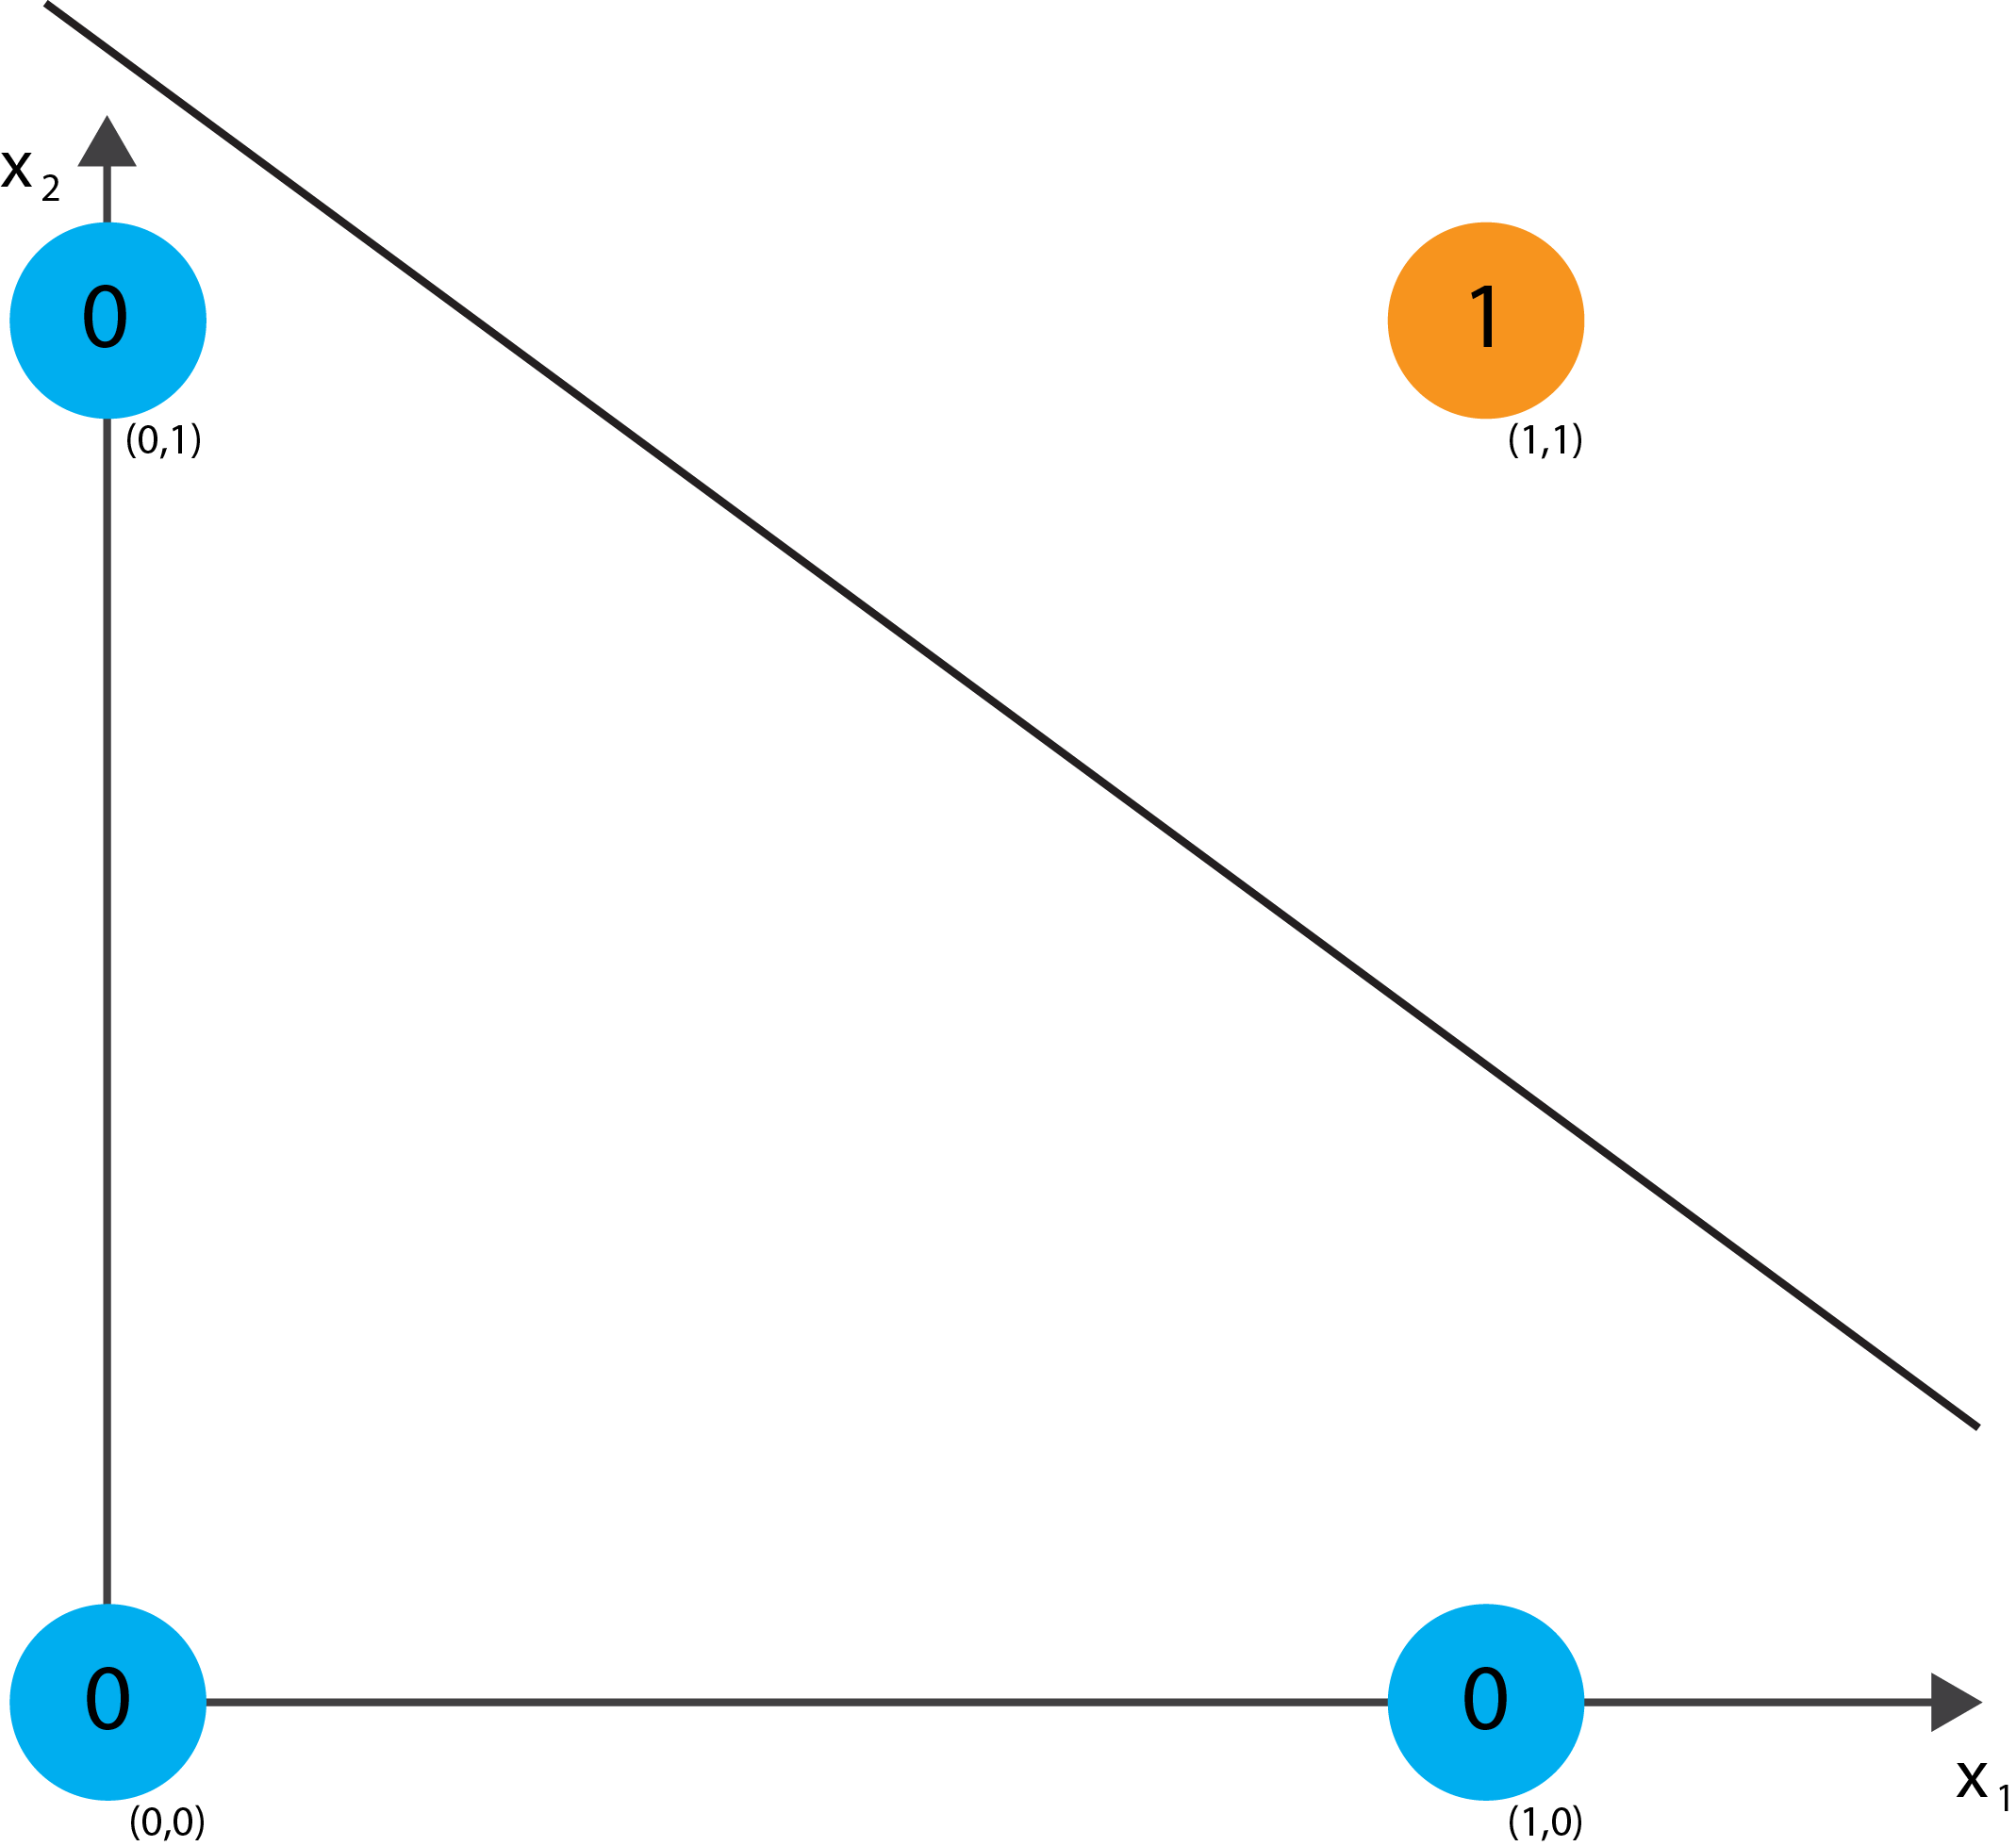
\includegraphics[width=0.22\textwidth]{svm/svm_and.png}}
    \caption{AND-Perzeptron}
    \label{fig:perceptron_and}
\end{figure}

Die jeweiligen Gewichtungen können so eingestellt werden, dass der Eingabevektor in einen bestimmten Ausgabevektor umgewandelt wird. 
Abb. \ref{fig:perceptron_and} zeigt, wie ein einfaches Perzeptron die UND-Funktion realisiert und visualisiert die Klassifizierungsentscheidung in einem Koordinatensystem. 

Einlagige Perzeptronen sind beschränkt auf die Lösung linear separierbarer Probleme. 
Ein einfaches XOR kann also nicht realisiert werden (Abb. \ref{fig:perceptron_xor}). 

\begin{figure}[htbp] \centering
    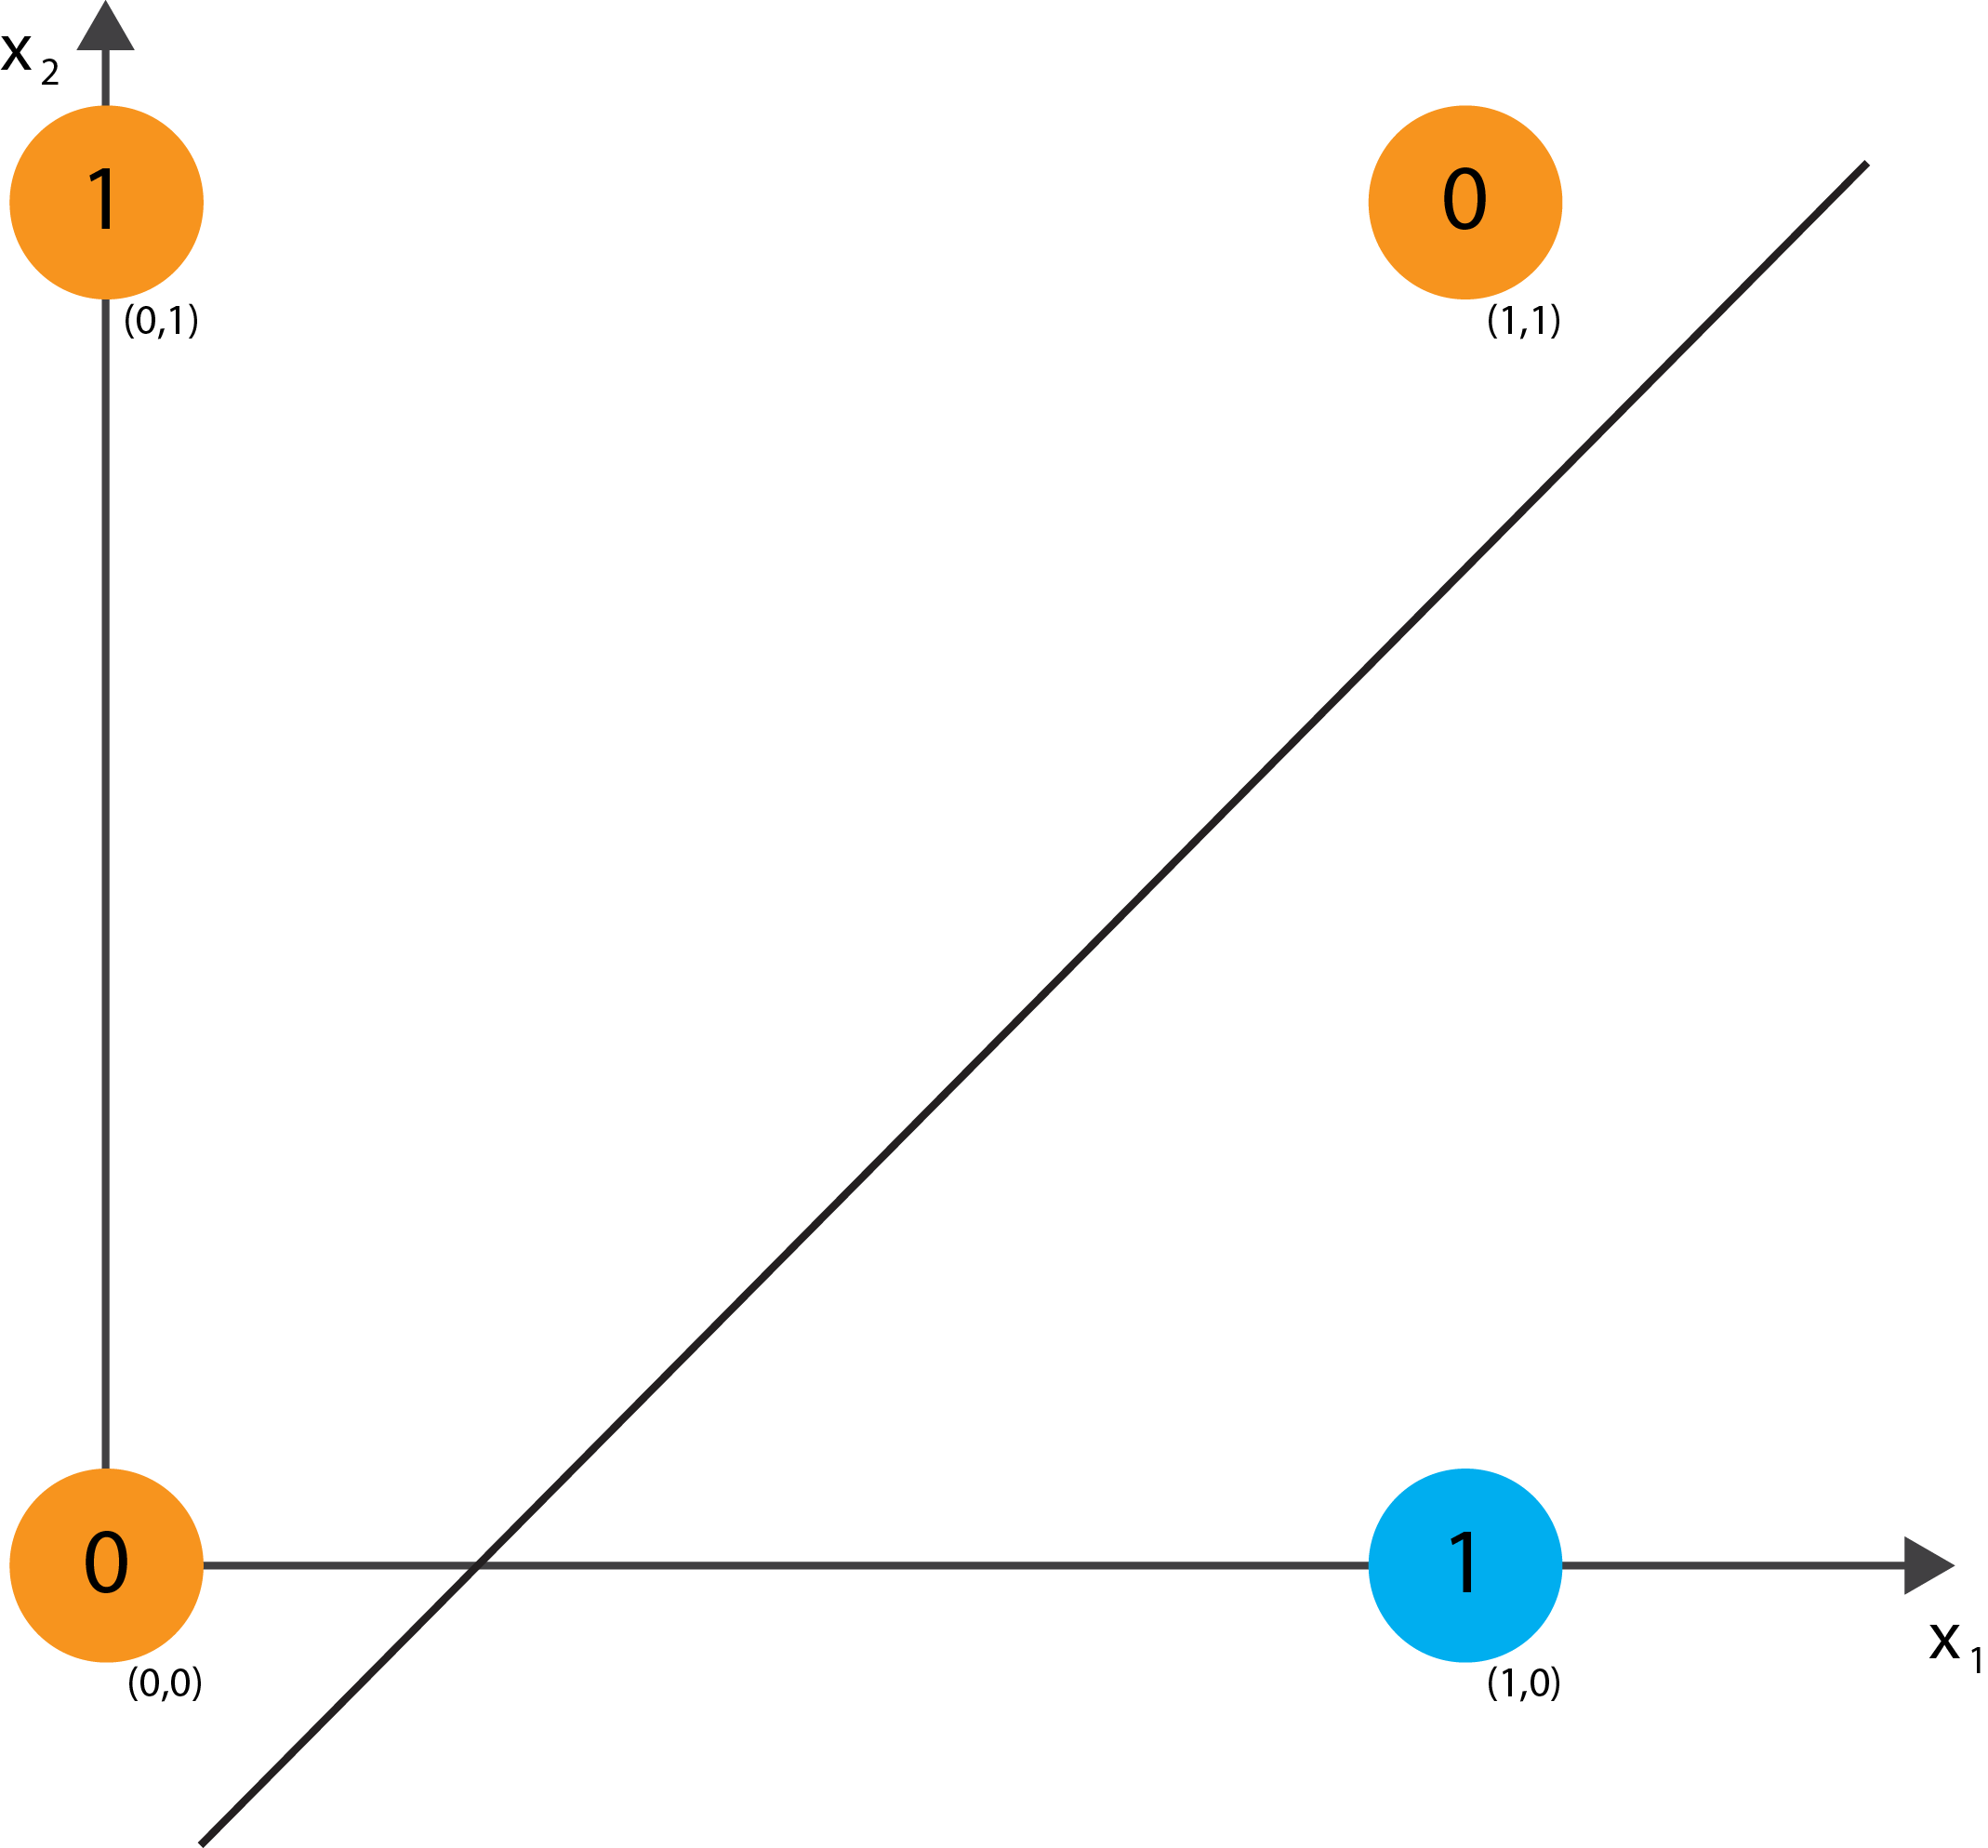
\includegraphics[width=0.22\textwidth]{svm/svm_xor.png}
    \caption{nichtlinear separierbares XOR}
    \label{fig:perceptron_xor}
\end{figure}


Mit einem Trick, der Erhöhung der Dimension, können mehrlagige Perzeptronen auch nichtlinear separierbare Probleme lösen. 
So lässt sich bspw. das XOR-Problem in einem 3-dimensionalen Raum durch eine Hyperebene trennen.

Die Wahl der richtigen Gewichte ist dabei nicht einfach, für komplexere Problemstellungen schier unmöglich. 
Um dennoch eine Problemlösung zu modellieren, die Eingaben richtig klassifiziert, gibt es einen Algorithmus, der die Gewichte automatisch anpasst.
Dieser Algorithmus setzt eine Trainingsmenge voraus, für dessen Eingabevektoren die zugehörigen Klassen bekannt sind. 
Durch Fehlerrückführung kann ein MLP trainiert werden und das Netz kann die gewünschten Muster nach einer kontrollierten Trainingsphase klassifizieren.

Knapp 40 Jahre Jahre später veröffentliche der sowjetisch-amerikanische Mathematiker Wladimir Wapnik \cite{Vapnik} das Prinzip der Support-Vector-Machines (SVM).

Im Gegensatz zu MLPs wird die Anpassung der Trennung nicht empirisch durch Trainingsmethoden, sondern durch die Datengrundlage mathematisch optimal ermittelt. 
Eine Erhöhung der Dimension ist nicht möglich, dennoch können SVMs auch nichtlinear separierbare Probleme lösen. 
Die Hauptidee dabei ist die Repräsentation der Daten zu verändern. 
Mit Hilfe des sogenannten Kernel-Tricks werden die Daten in einen höherdimensionalen Raum transformiert. 

Support Vector Machines erfreuen sich großer Beliebtheit, da sie in der Regel wesentlich performanter vernünftige Vorhersagen treffen können. Lediglich durch die Lokalisierung des Objekts im Koordinatensystem wird klassifiziert. Dadurch, dass eine trainierte SVM eine Trenngerade generiert, kann durch einfache Hilfsmittel aus der linearen Algebra die Position bestimmt werden. Es wird also entschieden, ob das zu klassifizierende Objekt "{}oberhalb"{} oder "{}unterhalb"{} der Trenngeraden liegt. Allerdings ist zu beachten, dass für sehr große Datenmengen die SVM eine sehr lange Trainingsphase benötigt, da der Algorithmus die Inversion der Eingabematrix benutzt. Das Bilden der inversen Matrix hat eine Laufzeit zwischen $\mathcal O(n^2)$ und $\mathcal O(n^3)$ und ist damit sehr aufwändig.


\subsection{Funktionsweise der SVM}

\subsubsection{Optimale Trennung}
Mit einem Satz von Merkmalsvektoren (Merkmalsraum) und dessen Klassenzugehörigkeiten $\{ (x_1, y_1), ..., (x_m, y_m) | x_i \in \mathcal{X}, y_i \in \{-1, 1\}, m \in \mathbb{N} \}$ wird eine mathematische Gerade errechnet,
die in einem Koordinatensystem betrachtet die Daten räumlich in zwei Klassen trennt. 



Die Gerade (Hyperebene im mehrdimensionalen Raum) trennt die Merkmalsräume bestmöglich und dient als Entscheidungsfunktion für die Klassifikation. Sie ist gegeben durch den Normalenvektor $w$ und dem sogenannten Bias $b$, dem Abstand der Ebene zum Ursprung. Diese Form erweist sich also besonders praktisch, da durch Einsetzen von $x$ der direkte Abstand zur Hyperbene resultiert.
Intuitiv ist klar, dass alle Punkte auf der Hyperebene selbst keinen Abstand haben, die Formel der Hyperebene (\ref{eq:svm_hyperplane}) lautet demnach: 
 
\begin{equation}
\label{eq:svm_hyperplane}
    \mathcal{H}: \{ x \,|\, \langle w,x \rangle + b = 0 \}
\end{equation}
 
Allein durch das Vorzeichen der Entscheidungsfunktion ordnet die \ac{SVM} die Eingabe einr Klasse zu. Dabei können nur zwei Klassen  prognostiziert werden. Die Klasse gehört demnach entweder zur Klassenmenge \ref{eq:svm_decision0} oder zu \ref{eq:svm_decision1}.

\begin{eqnarray}
    \mathcal{C}_{-1}: \{ c \,|\, sign(\langle w,x \rangle + b) = -1 \} \label{eq:svm_decision0} \\
    \mathcal{C}_1: \{ c \,|\, sign(\langle w,x \rangle + b) = 1 \} \label{eq:svm_decision1}
\end{eqnarray}

Die nächstliegenden Vektoren zur Trenngeraden werden als Stützvektoren, der Abstand als Margin $M$ bezeichnet (Abb. \ref{fig:svm_separator}). 

\begin{figure}[htbp] \centering
    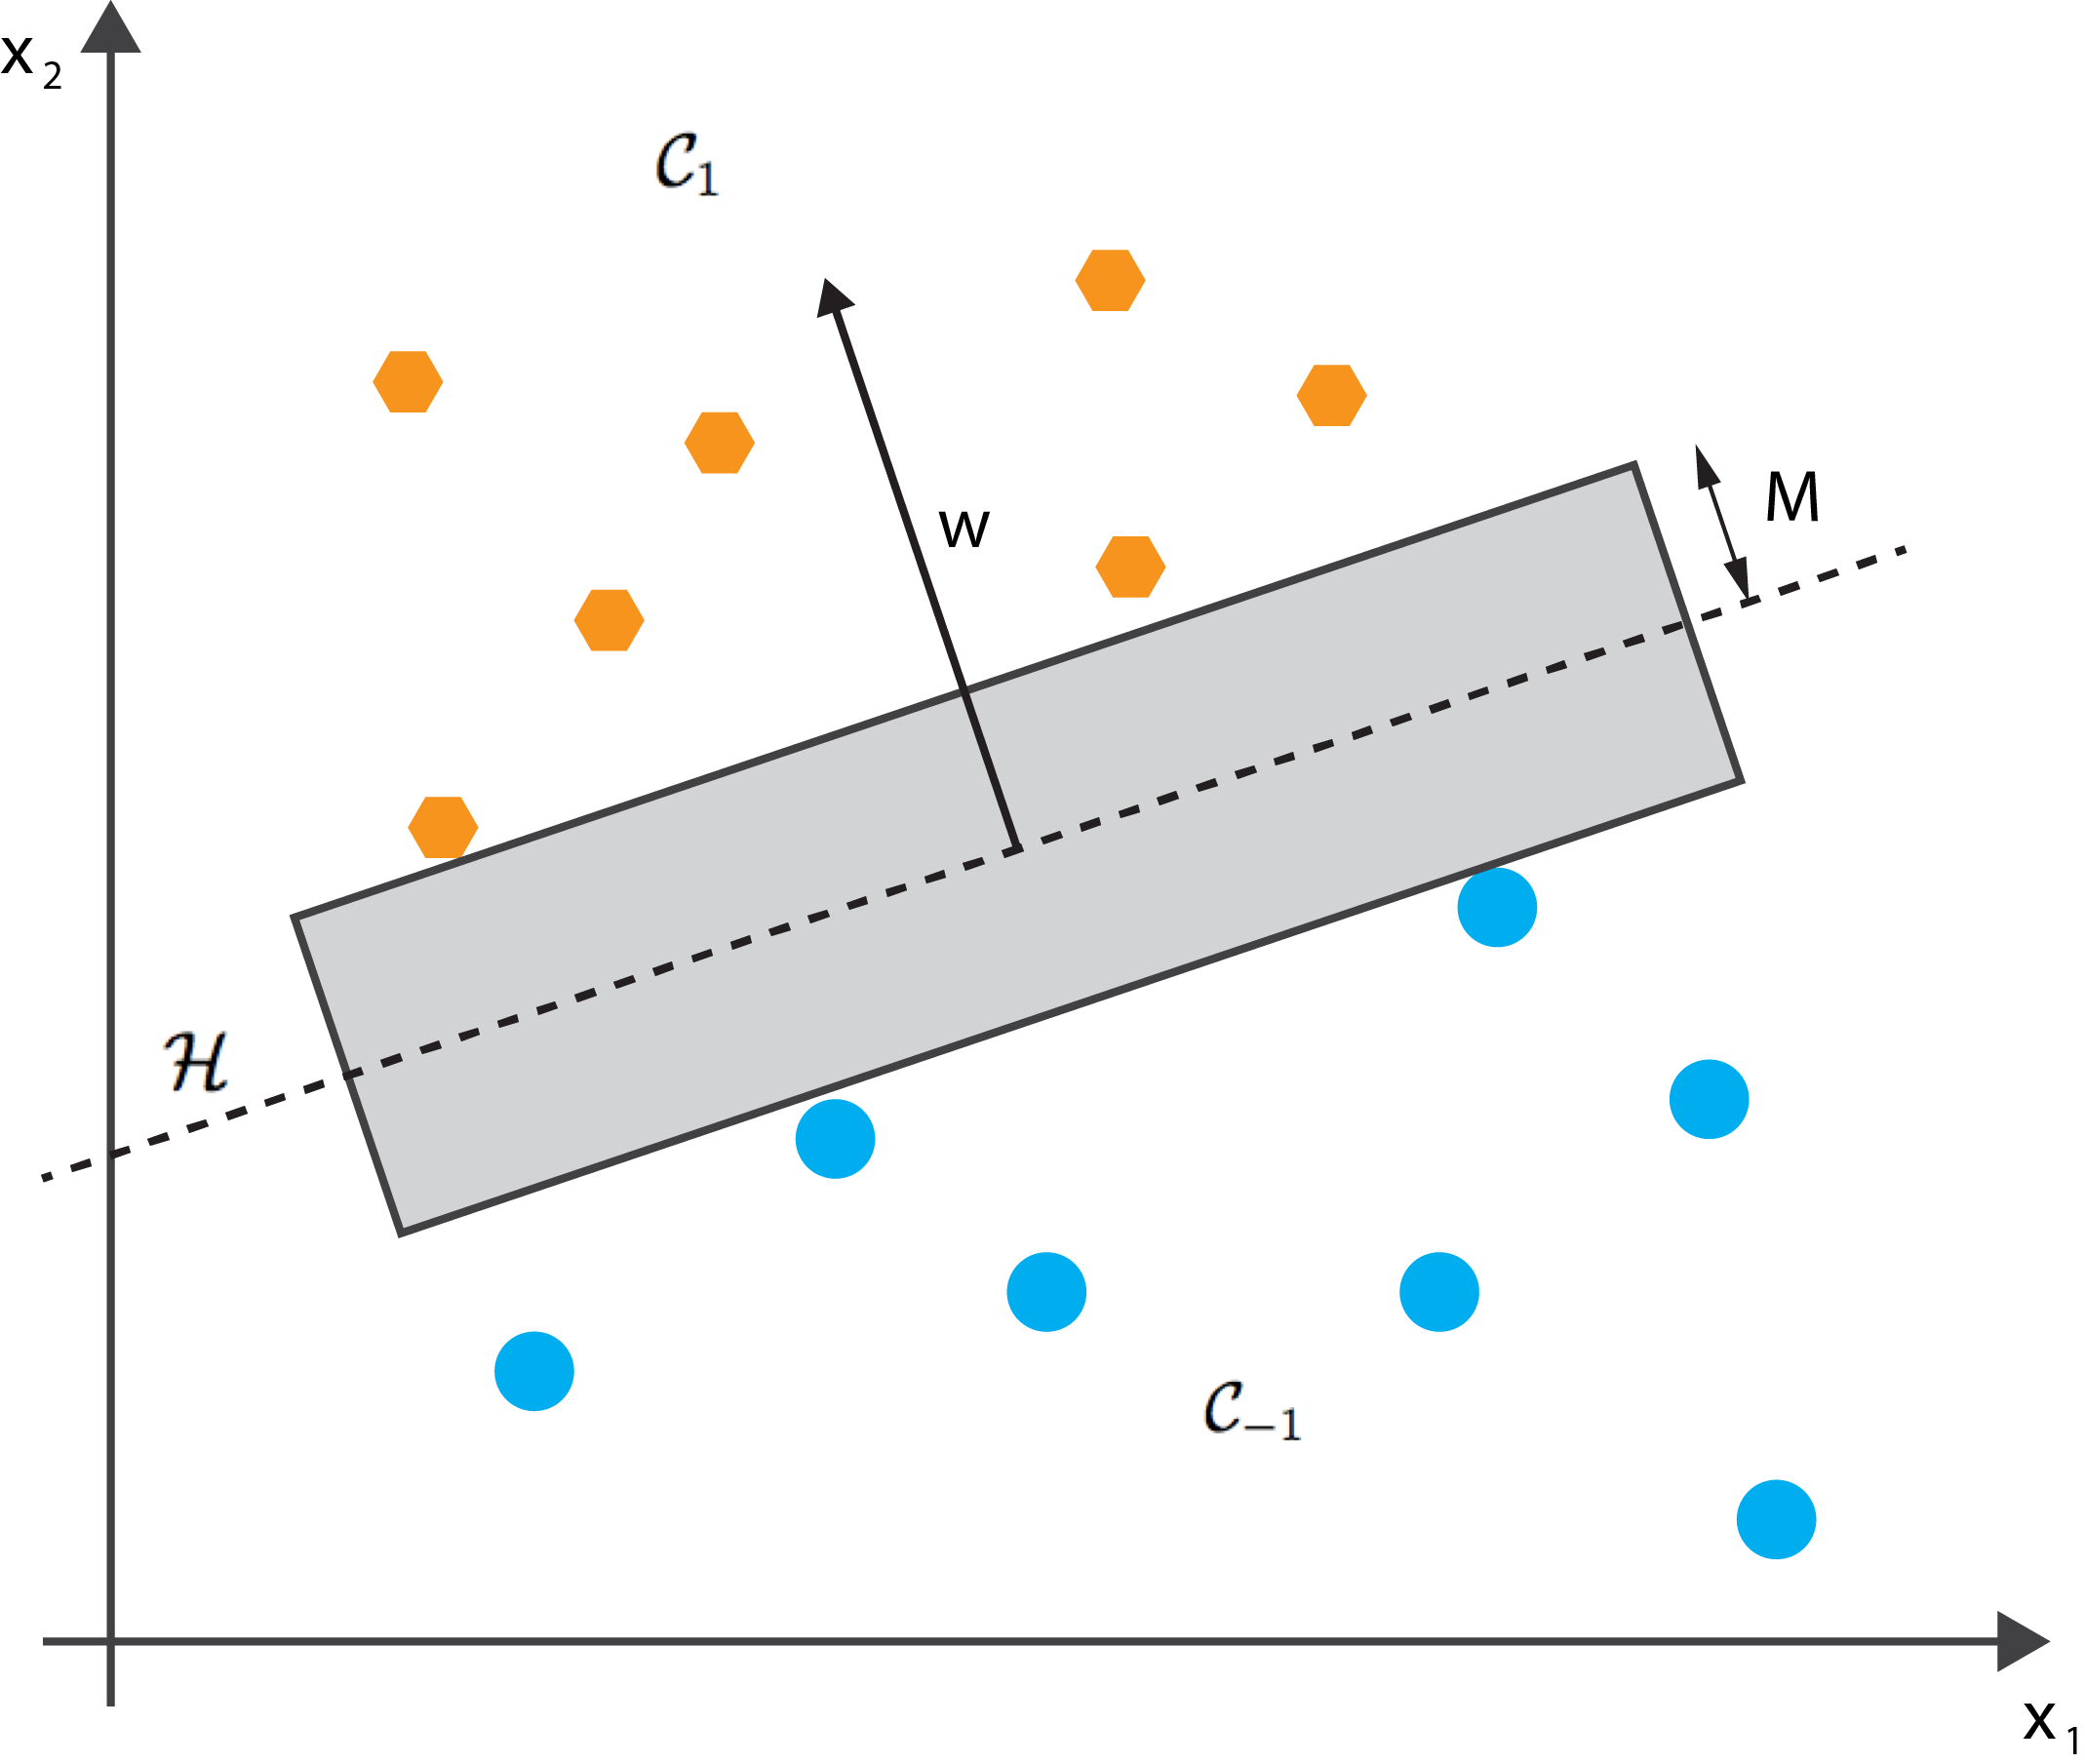
\includegraphics[width=0.3\textwidth]{svm/svm_overview.png}
    \caption{Trenngerade einer SVM}
    \label{fig:svm_separator}
\end{figure}

Die Stützvektoren bilden das tragende Konstrukt der Entscheidungsfunktion. 
Alle andere Merkmalsvektoren haben keinen Einfluss auf die Trennung, was die Namensgebung der Stützvektoren begründet. 
Das macht die \ac{SVM} zu einem sehr transparenten und performantent Klassifikator. 


\subsubsection{Kernel-Trick}
Es ergeben sich Unregelmäßigkeiten bei der Lösung von nichtlinear separierbaren Probleme und der Klassifikation von mehr als 2 Klassen.
Im Gegensatz zu den MLPs kann man mit der Erhöhung der Dimension diesen Umstand nicht umgehen. 
Die \ac{SVMs} setzen in diesem Falle auf die Transformation der Datenrepräsentation. 
Mit Hilfe von Kernfunktionen (\ref{eq:svm_kernel_function}) lassen sich Daten von $\mathbb{R}^n$ in einen höherdimensionalen Raum $\mathbb{R}^h$ transformieren in dem sie linear separierbar erscheinen (Abb. \ref{fig:svm_kernel}). 

\begin{equation}
\label{eq:svm_kernel_function}
\begin{split}
    \phi : & \mathbb{R}^n \to \mathbb{R}^h \\
    & x \mapsto \phi(x)
\end{split} 
\end{equation}

\begin{figure}[htbp] \centering
    \subfigure[Datenpunkte $x$ nichtlinear separierbar]{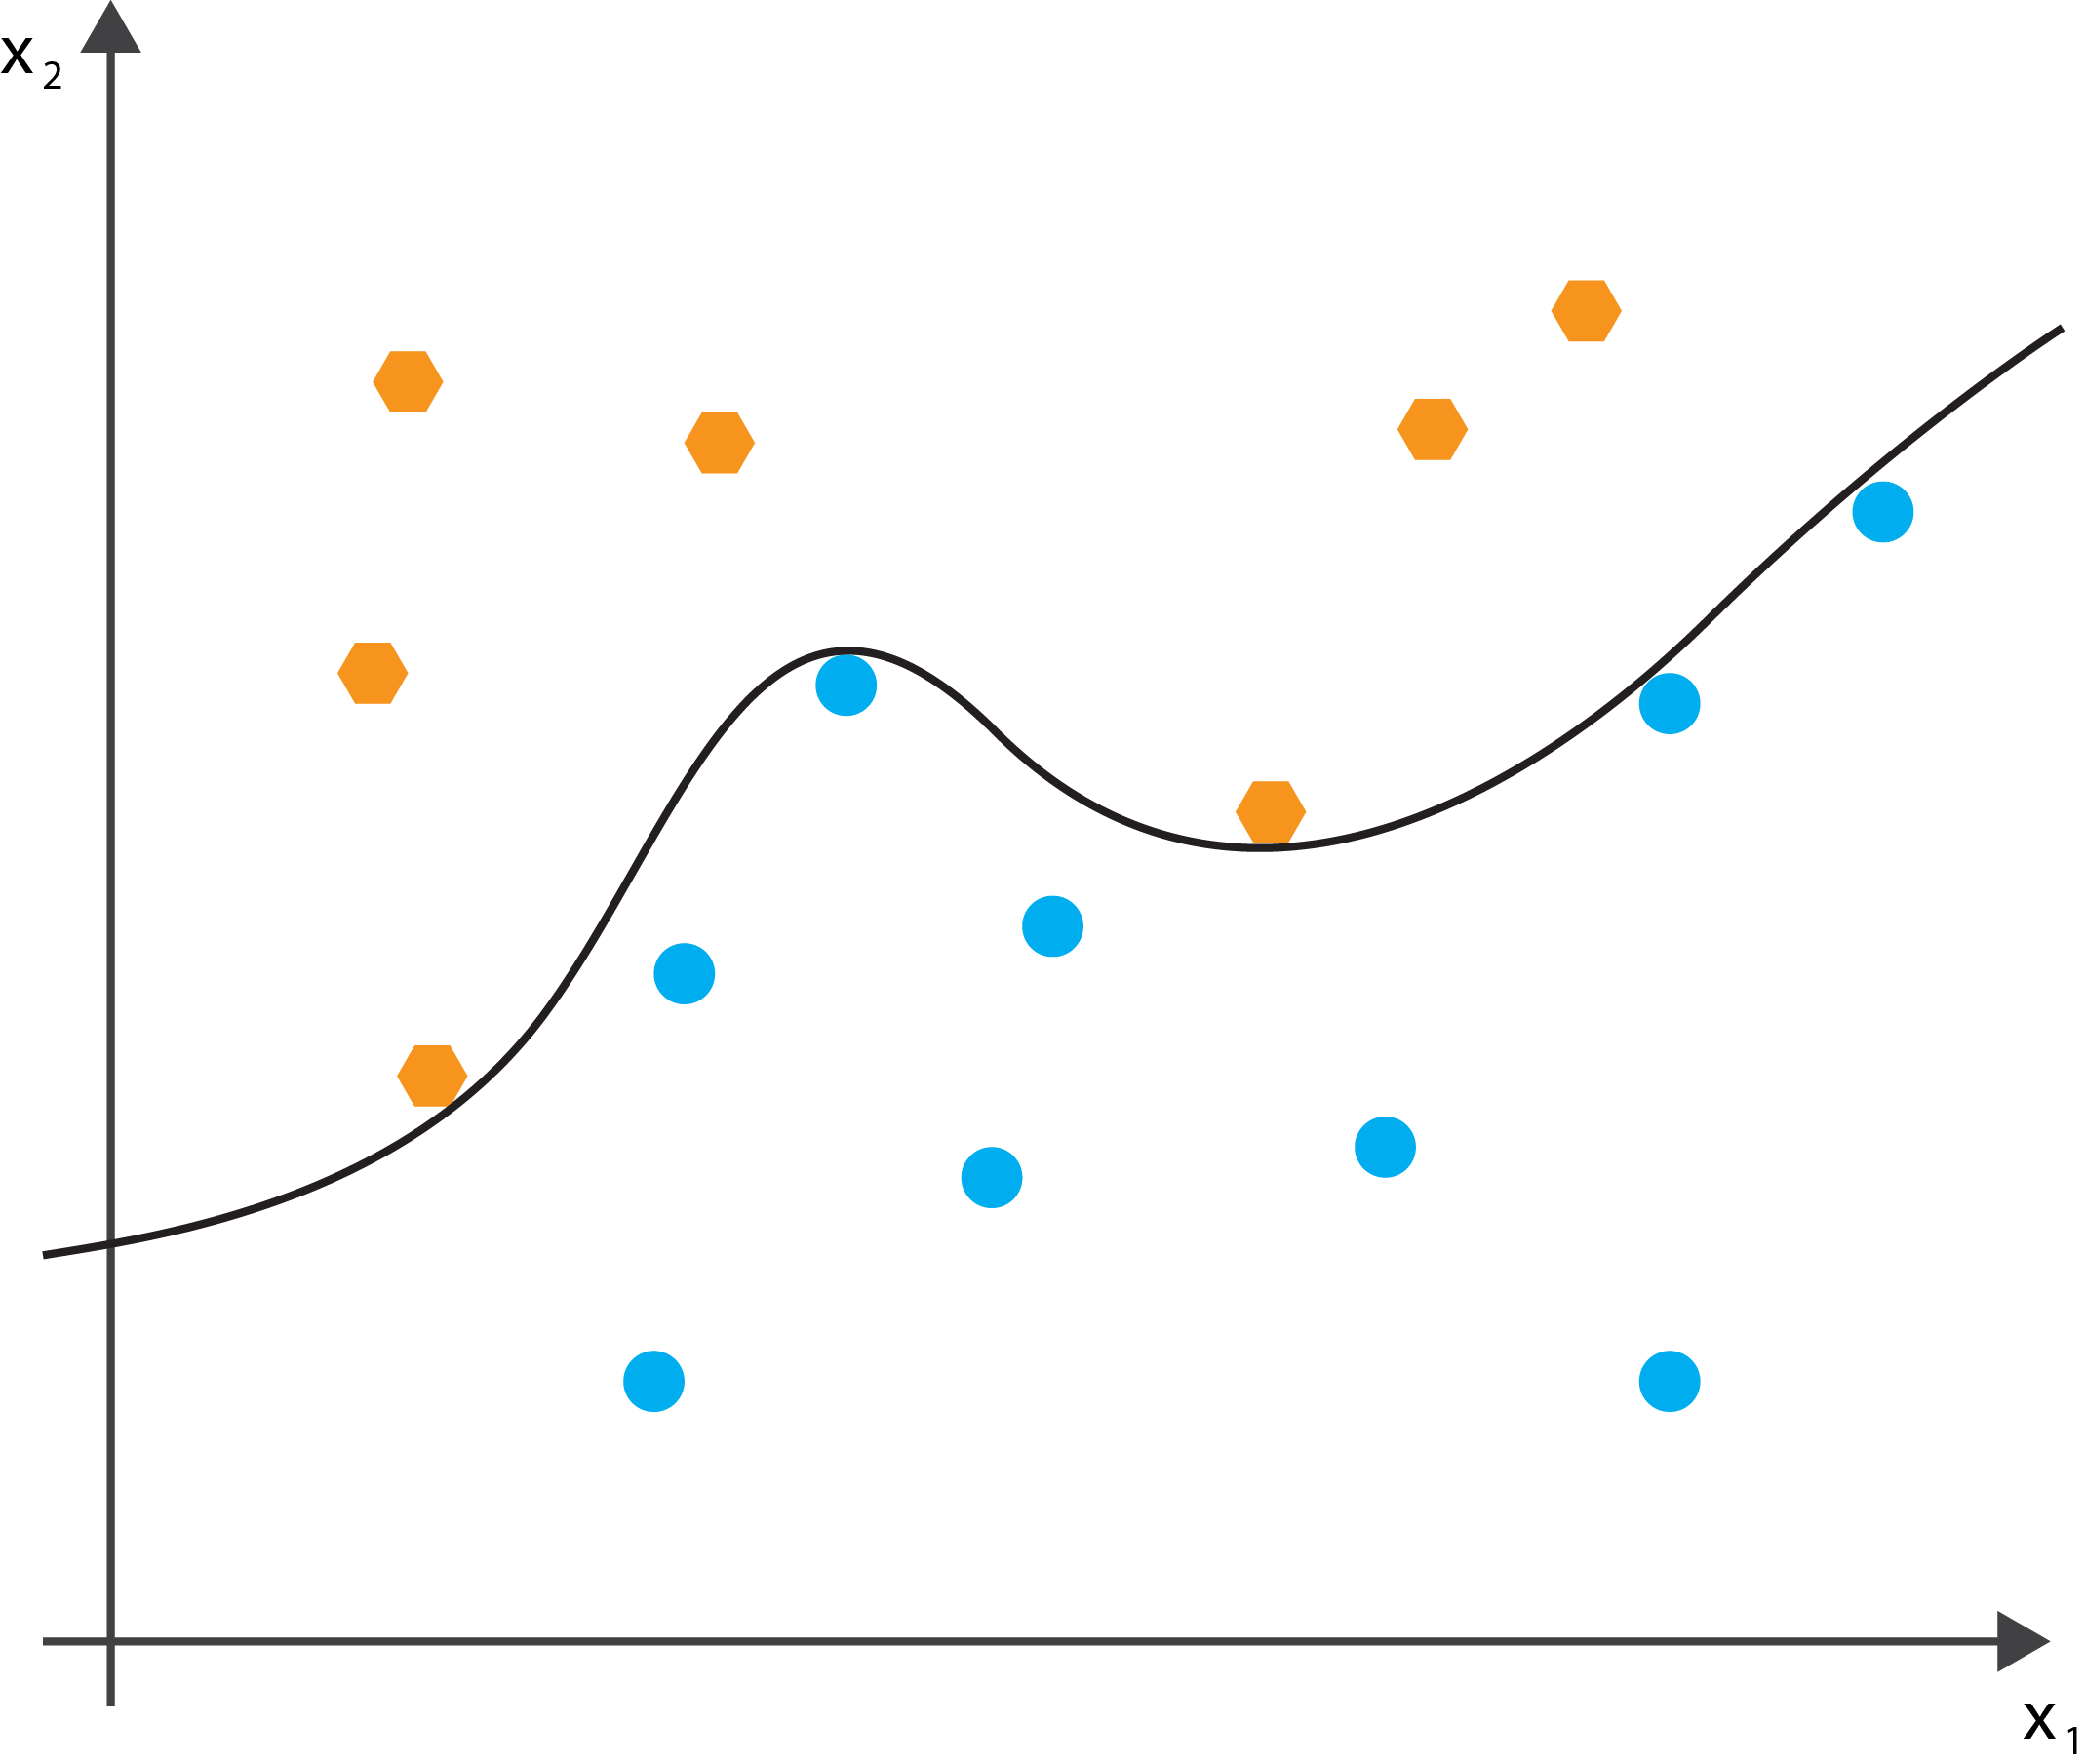
\includegraphics[width=0.22\textwidth]{svm/svm_fitting-line.png}}
    \subfigure[transformtierte Datenpunkte $\phi(x)$ linear sepraierbar]{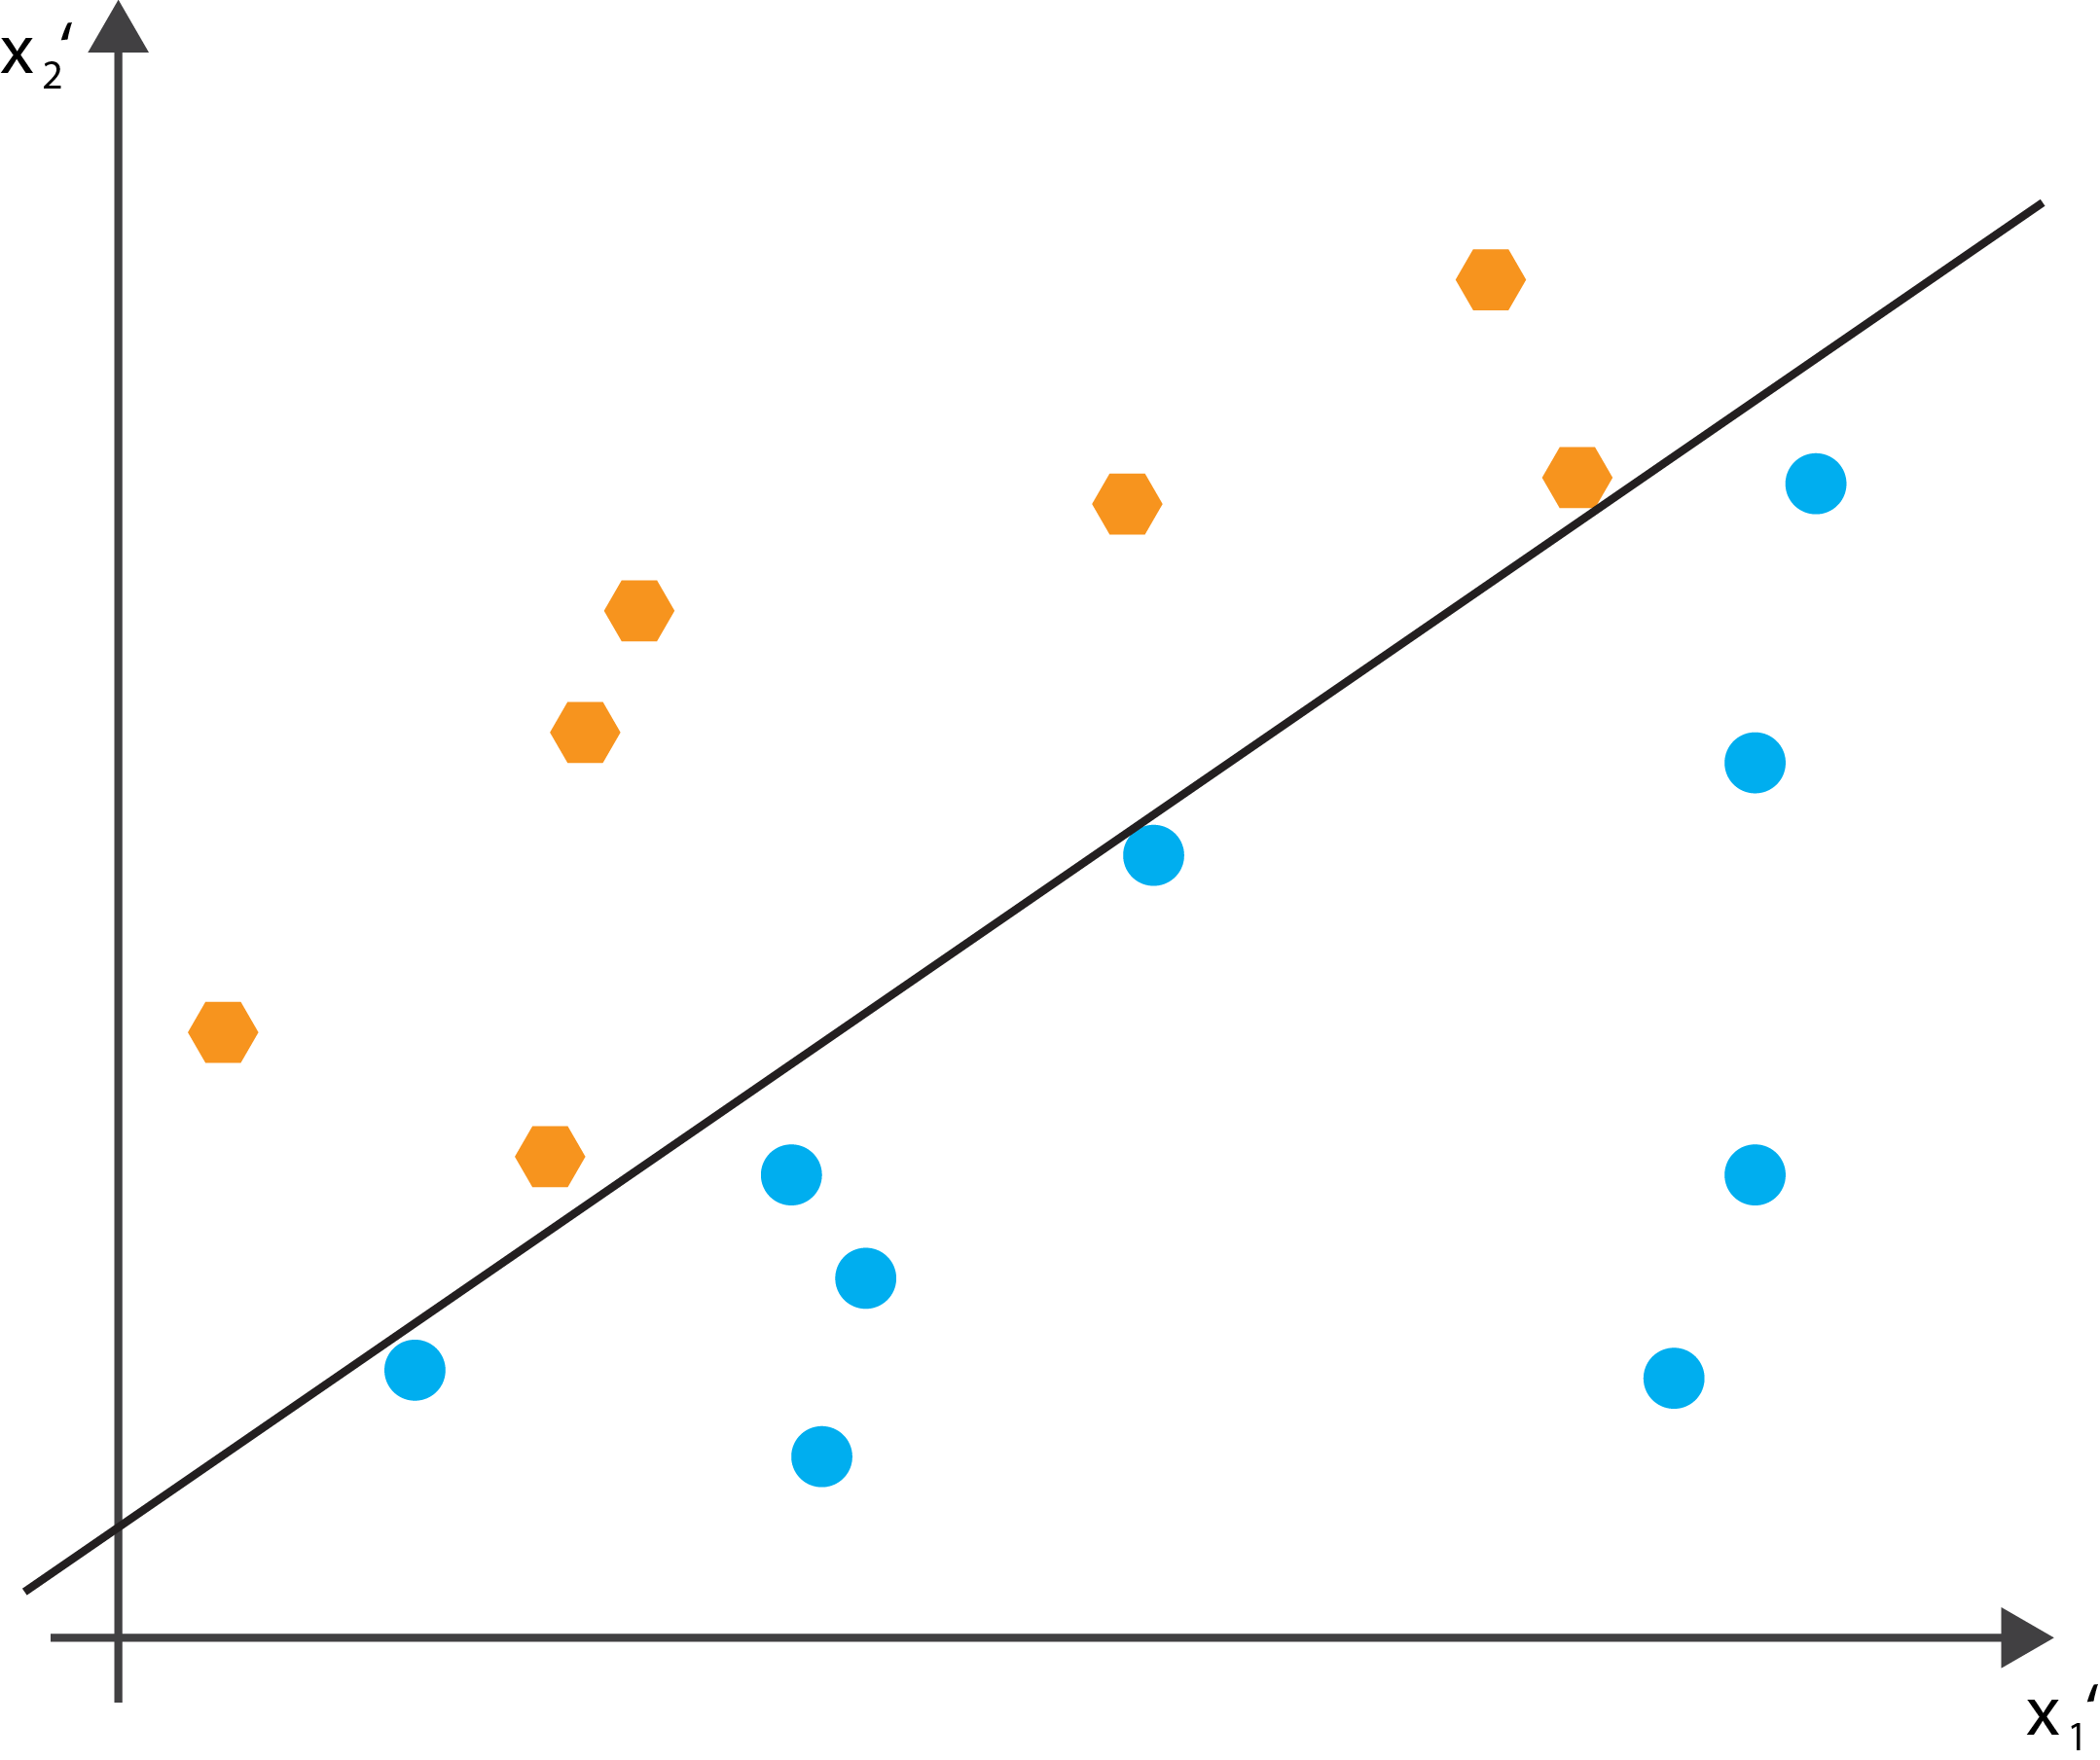
\includegraphics[width=0.22\textwidth]{svm/svm_linear-fitting.png}}
    \caption{Kernfunktion $\phi$}
    \label{fig:svm_kernel}
\end{figure}

Als Bedingung des Raums $\mathbb{R}^h$ gilt, dass das Skalarprodukt erklärt ist. 
Wir haben nach der Transformation also die neue Form \ref{eq:svm_kern_tranformation}. 
In der neuen Form müssen wir nun das Skalarprodukt $\langle\phi(w),\phi(x)\rangle$ ausrechnen, was sehr schwierig (bzw. unmöglich) ist, wenn die Dimension von $\mathbb{R}^h$ zu groß wird.

\begin{equation}
\label{eq:svm_kern_tranformation}
    \mathcal{C}: \{ c_i \,|\, sign(\langle \phi(w),\phi(x) \rangle + b) = i \}
\end{equation}


Dadurch, dass die Trainingspunkte $x$ nur in Skalarprodukten auftauchen, können wir uns des Kernel-Tricks bedienen.
Kernfunktionen, die in $\mathbb{R}^n$ leben, zeichnen sich durch eine spezielle Eigenschaft aus, da sie sich verhalten wie ein Skalarprodukt in $\mathbb{R}^h$ (\ref{eq:svm_kern_trick}). 

\begin{equation}
\label{eq:svm_kern_trick}
    \mathcal{K}(w,x) = \langle\phi(w),\phi(x)\rangle
\end{equation}

Es kann also das Skalarprodukt $\langle\phi(w),\phi(x)\rangle$ in $\mathbb{R}^h$ ausgerechnet werden, ohne die Daten mittles $\phi$ zu transformieren. 
Das Beispiel \ref{fig:ex_kernel} verdeutlicht die Anwendung des Kernel-Tricks  anhand einer polynomiellen Kernfunktion:

\renewcommand{\figurename}{Bsp.}
\begin{figure}[htbp]
\begin{equation*}
\label{eq:svm_kernel_example}
\begin{split}
    \text{Seien } w,x & \in \mathbb{R}^2 \text{ und}\\
    \phi : & \mathbb{R}^2 \to \mathbb{R}^3\\
    & \begin{pmatrix}
    x_1 \\
    x_2
    \end{pmatrix}
    \mapsto
    \begin{pmatrix}
    x_1^2 \\
    \sqrt{x_1x_2} \\
    x_2^2
    \end{pmatrix}\\
    \text{dann ist:} &\\
    \langle \phi(w),\phi(x) \rangle = & \:\langle \begin{pmatrix}
    w_1^2 \\
    \sqrt{w_1w_2} \\
    w_2^2
    \end{pmatrix},
    \begin{pmatrix}
    x_1^2 \\
    \sqrt{x_1x_2} \\
    x_2^2
    \end{pmatrix} \rangle \\
    \\
    = & \:w_1^2x_1^2 + 2 w_1x_1w_2x_2 + w_2^2x_2^2 \\
    \\
    = & \:(w_1x_1 + w_2x_2)^2 \\
    \\
    = & \:\langle w,x \rangle^2 \overset{\text{(def)}}= \mathcal{K}(w,x)
\end{split}
\end{equation*}
    \caption{Beispiel einer Kernfunktion}
    \label{fig:ex_kernel}
\end{figure}
\renewcommand{\figurename}{Abb.}

Nicht jede beliebige Funktion ist eine Kernfunktion. Kernfunktionen müssen die Bedingungen nach Satz von Mercer \cite[S. 127]{Marsland} erfüllen. 
Gängige Kernfunktionen sind:
\begin{itemize}
\item{linear: $\mathcal{K}(w,x) = \langle w,x \rangle$}
\item{polynomiell: $\mathcal{K}(w,x) = (\gamma\langle w,x \rangle+c_0)^d$}
\item{radial basis function: $\mathcal{K}(w,x) = exp(- \gamma \|w - x \| ^2)$}
\end{itemize}

\newpage

\subsubsection{Klassifikation von mehreren Klassen}

Da die \ac{SVM} als binärer Klassifikator entwickelt wurde, müssen für eine Klassifikation von mehr als zwei Klassen Strategien entwickelt werden, um das Prinzip der \ac{SVM} zu erweitern. 
Ein Verfahren ist die "{}Einer gegen den Rest"{}-Klassifikation. 
Bei dieser Technik wird für jedes zu klassifizierende Objekt eine binäre \ac{SVM} trainiert. 
Für jede \ac{SVM} wird eine Klasse separiert, die anderen Klassen werden nicht unterschieden und als negative Beispiele zu einer Restklasse definiert. 
Die Vorraussage eines Objektes ergibt sich aus der Auswertung aller \ac{SVMs}. 
Es ist nun möglich, dass mehrere \ac{SVMs} eine positive Klassenzuordnung feststellen nicht die Restklasse klassifizieren. 
In diesem Fall entscheidet sich das "{}Einer gegen den Rest"{}-Verfahren für die Klasse, dessen \ac{SVM} die höchste Ausgabe erzeugt (winner-takes-all). 
Als höchstes Ergebnis wird der größte Abstand zur Trennhyperebene angenommen. 
Offensichtlich erhöht sich die Laufzeit der Trainingsphase mit der Anzahl der Klassen $|\mathcal{C}|$. 
Glücklicherweise beeinflusst das nicht die Laufzeitanalyse in der $\mathcal{O}$-Notation (\ref{eq:svm_winner_runtime}). 

\begin{equation}
\label{eq:svm_winner_runtime}
    |\mathcal{C}| \cdot \mathcal{O}(n) = \mathcal{O}(|\mathcal{C}| \cdot n) =  \mathcal{O}(n)
\end{equation}

Sind die SVMs trainiert, beeindrucken sie durch rasante Klassifikation. 
Dies ermöglicht uns eine echtzeitnahe Gestenerkennung.



\newpage 
\subsection{Anwendung auf das Projekt}
Für das Projekt wird eine \ac{SVM} trainiert, die mit nur geringfügig den Standardwerten des verwendeten Python-Moduls abweichenden Parametern trainiert wird. 
Für das Training erwartet die \ac{SVM} neben einem Eingabevektor mit 320 Werten noch die dazugehörige Klasse; die Länge des Eingabevektors lässt sich allerdings über einen entsprechenden Parameter in einer separaten Konfigurationsdatei noch halbieren.
Während der Live-Klassifikation von Gesten, beziehungsweise deren Eingabevektoren, wird die trainierte \ac{SVM} für die Erkennung verwendet.
Natürlich müssen diese Eingabevektoren in ihrer Dimension den Trainingsdaten entsprechen.

Der nächste Abschnitt widmet sich der Datenaufbereitung, insbesondere der Reduzierung der Dimension eines Eingabevektors und der entsprechenden Vorverarbeitung.

\subsubsection{Datenaufbereitung}\label{sec:svm_data} 
In \autoref{sec:intro} wurde die Aufnahme und die generelle Vorverarbeitung der Daten bereits erläutert, bevor diese an die entsprechenden Klassifikatoren weitergeleitet werden.
Da jeder Klassifikator aufgrund seiner Funktionsweise unterschiedlich mit den Eingabedaten arbeitet, ist eine entsprechende und auf den jeweiligen Klassifikator angepasste Datenaufbereitung notwendig.
Gleichzeitig kann durch eine entsprechende Vorverarbeitung gegenüber unverarbeiteten Daten das Problem der Klassifikation von unterschiedlichen Datensätzen verallgemeinert und somit die Trainingszeit verringert werden.
Dieser Abschnitt befasst sich mit der spezifischen Datenaufbereitung für den \ac{SVM} Klassifikator.

\paragraph{Eingabevektordimensionsreduzierung}\label{sec:svm_reduce}$\;$ \\
Bei der Betrachtung der Trainingsdaten, die jeweils aus insgesamt 32 Frames zu je 64 Werten bestehen, wird offensichtlich, dass die durch den Doppler-Effekt verursachten Frequenzverschiebungen in einem begrenzten Umfeld der Referenzfrequenz von $18\text{,}5\text{ kHz}$ herum sattfinden.
Zudem stellt sich heraus, dass nur ein Bruchteil der ursprünglich veranschlagten 32 Frames pro Geste relevante Informationen enthalten, da die Ausführung einer Geste meist zwischen 8 und 20 Frames dauert und nur innerhalb dieser Frame-Anzahl Frequenzverschiebungen verursacht.
Aufgrund dieser beiden Gründe werden im ersten Schritt der Reduzierung der verwendete Wertebereich eines Frames von 64 auf 40 verkleinert und im nächsten Reduzierungsschritt sowohl für das Training der \ac{SVM}, als auch für die Live-Klassifikation, nur 16 Frames pro Geste verwendet. 

Die dritte Reduzierung wird mittels der Addition benachbarter Frames erzielt, so dass letztlich nur noch jeweils 8 Frames zu je 40 Werten pro Datensatz/Geste existieren.
Im Anschluss erfolgt die Transformation in ein eindimensionales Array mit insgesamt 320 Werten, welches als Eingabevektor für die \ac{SVM} dient.
Gegenüber der ursprünglichen Gesamtanzahl von 2048 Werten pro Datensatz wurde mittels der Vorverarbeitung die Dimension eines Eingabevektors um etwa den Faktor $6\text{,}5$ verringert.
Eine weitere Reduzierung um den Faktor 2 ist möglich, sofern nur jeder zweite Wert des Eingabevektors verwendet werden soll.

\begin{figure*}[htbp] \centering
    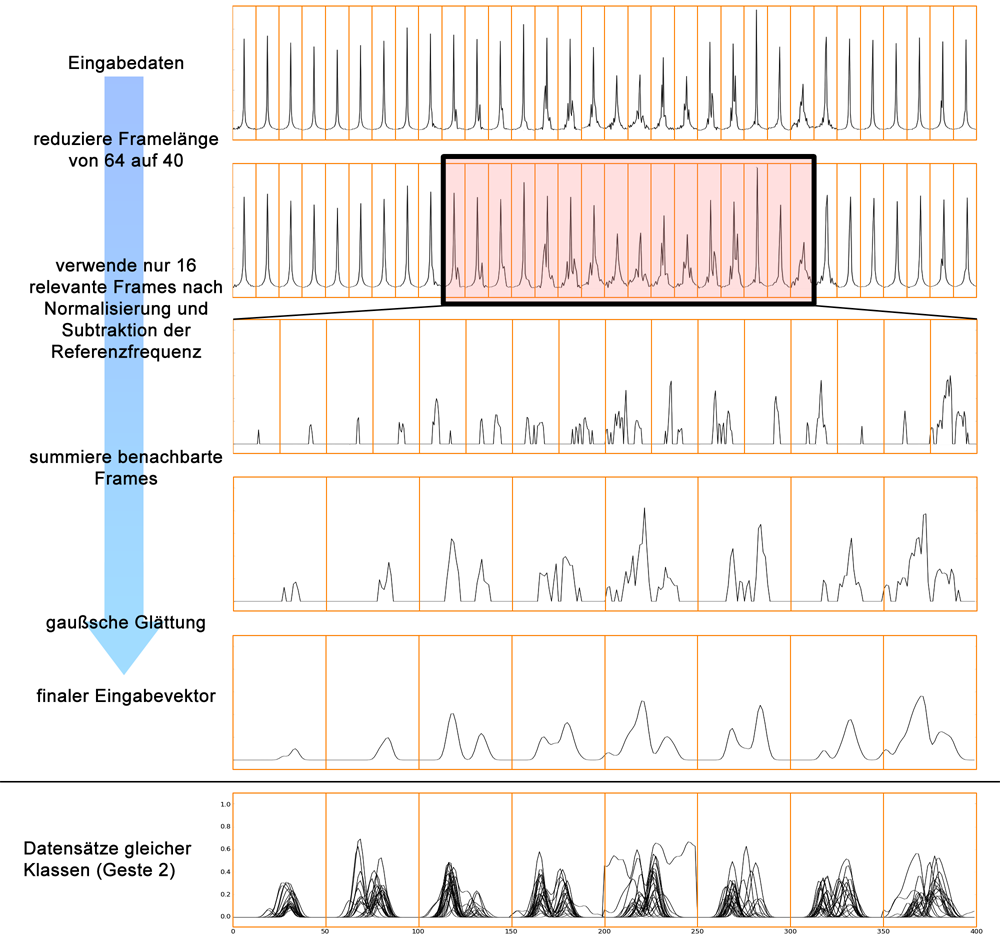
\includegraphics[width=0.65\textwidth]{svm/svm_preprocessing_steps.png}
    \caption{Vorverarbeitungsschritte}
    \label{fig:svm_preprocessing_steps}
\end{figure*}

\paragraph{Vorverarbeitung}\label{sec:svm_preprocess}$\;$ \\\\
Die Reduzierung der Eingabevektordimension und die vorverarbeitenden Schritte sind zwei notwendige Handlungen, die sich in der Implementierung nicht trennen lassen, allerdings lassen sie sich in ihrer Beschreibung gut separieren.
Unmittelbar nach dem ersten Reduzierungsschritt wird jeder einzelne Frame normalisiert und die Referenzfrequenz subtrahiert.
Da trotz Subtraktion der Referenzfrequenz teilweise noch sehr feines Rauschen in den Daten vorhanden sein kann, werden Werte unterhalb eines festgelegten Schwellenwerts auf 0 gesetzt.
Die ersten 16 Frames, die relevante Informationen enthalten (Frame-Maximalwert > 0), werden für den dritten Reduzierungsschritt verwendet.
Optional und standardmäßig aktiviert wird eine eindimensionale Gauß'sche Filterung zur Glättung der Werte als abschließender Vorverarbeitungsschritt angewandt.

\subsubsection{Implementierung}\label{sec:svm_implementation}
Aufgrund des Einsatzes von verschiedenen Klassifikatoren ist ein gemeinsames Interface für alle Klassifikatoren vorhanden, welches von jedem Klassifikator -- allerdings unterschiedlich -- implementiert ist. 
Dabei handelt es sich um die abstrakte Klasse \texttt{IClassifier}, die von der \ac{SVM}--Klasse im Modul \texttt{svm.py}  implementiert werden muss.

\begin{lstlisting}[float=*,language=Python,caption={classify},label={lst:svm_classify}]{lst:svm_classify}
import numpy as np
import svm_appstarter as Starter
appstarter = Starter()

def classify(data):
	frame = preprocess_frame(slice_frame(data),ref_frequency_frame)
	datalist.append(frame)
	datanum += 1
	
	if timeout < framerange/2:
		timeout += 1
		if timeout == framerange/2:
			print "..."
	
	if np.amax(frame) > 0.0 and gesturefound == 0 and timeout == framerange/2:
		gestureindex = datanum
		gesturefound = 1
		
	if gestureindex + ramerange == datanum and gesturefound == 1:
		gesturefound, gestureindex, timeout = 0, 0, 0
		if new_preprocess:
			current_frameset = [frame for frame in datalist[-framerange:] if np.amax(frame) > 0]
			while len(current_frameset) < framerange/2:
				current_frameset.append(np.zeros(wanted_frames))
			current_frameset = np.asarray(current_frameset)
			relevant_frames = np.asarray(list(current_frameset[:framerange/2:2] + current_frameset[1:framerange/2:2])).reshape(wanted_frames*framerange/4,)
			if smooth:
				if use_each_second:
					normalised_gesture_frame = gaussian_filter1d(relevant_frames, 1.5)[::2]
				else:
					normalised_gesture_frame = gaussian_filter1d(relevant_frames, 1.5)
			else:
				normalised_gesture_frame = relevant_frames
			
			try:
				appstarter.controlProgram(classifier.predict(normalised_gesture_frame)[0])
			except:
				print "some error occured =("
			
	if datanum > framerange:
		del datalist[0]
\end{lstlisting}


Für die Implementierung der \ac{SVM}--Klasse wird die Python-Bibliothek \textit{scikit-learn} verwendet. 
Die Bibliothek stellt neben einer Vielzahl von weiteren Modulen und Klassen unter anderem auch eine Implementierung einer \ac{SVM} zur Verfügung.
Für grundlegende Matrizenberechnungen in den Modulen \texttt{svm\_dataloader.py} und \texttt{svm\_preprocessor.py} werden die Python-Bibliotheken \textit{NumPy} und \textit{SciPy} verwendet. 
\textit{NumPy} zeichnet sich vor allem durch effiziente Berechnungsoperationen und eine Vielzahl an nützlicher Funktionen aus, die durch das Erweiterungsmodul \textit{SciPy} um weitere sinnvolle Methoden ergänzt werden.
Zusätzlich findet das in der Python-Installation enthaltene \textit{os}-Modul Einsatz, um grundlegende Dateipfadkonkatenationen zu bewerkstelligen.
Letztendlich wird das ebenfalls standardmäßig in der Python-Installation enthaltene \textit{subprocess}-Modul verwendet, um mittels erkannter Gesten verschiedene Programme starten und beenden zu können.


Die Methode \textit{classify} erhält von dem Hauptprogramm jeweils einzelne Frames zu je 64 Werten, die sich innerhab des Frequenzbereichs um die Referenzfrequenz von $18\text{,}5\text{ kHz}$ befinden.
Anschließend wird direkt der erste beschriebene Vorverarbeitungsschritt pro übergebenem Frame ausgeführt, die in einer globalen Liste \texttt{datalist} abgespeichert werden.
Mittels einer Abfrage, ob der Frame überhaupt relevante Informationen besitzt, wird der Gestenanfang erkannt und der entsprechende Index der Liste \texttt{datalist} gespeichert.
Sobald 32 weitere Frames in dieser Liste abgespeichert worden sind, werden die 16 relevanten Frames herausgesucht und mittels der weiteren Vorverarbeitungsschritte zu einem Eingabevektor mit 320 Werten transformiert.
Der Eingabevektor wird dem Klassifikator übergeben, welcher als Rückgabewert die entsprechende Gestennummer zurückliefert, die er dem Eingabevektor zugeordnet hat.
Gleichzeitig dient diese Gestennummer zur Steuerung von diversen Programmen.
So kann mittels der Geste 0 der Notepad-Editor geöffnet und mittels der Geste 1 wieder beendet werden.
Diese Funktionalität ist einem separaten Modul \texttt{svm\_appstarter.py} ausgelagert.




\subsubsection{Training}
Die Trainingsmethode greift auf die eingelesenen und vorverarbeiteten Datensätze und die entsprechenden Klassenzugehörigkeiten zu und übergibt sie der \texttt{fit()}-Methode der \ac{SVM}-Klassifikatorimplementierung.
Dieser Klassifikator wurde davor bereits mit den in der Konfigurationsdatei festgelegten Parametern initialisiert.
Nach dem Training wird eine globale Referenz auf die trainierte \ac{SVM} gespeichert.
Gleichzeitig wird die trainierte \ac{SVM} auf der Festplatte für spätere Aufrufe komprimiert gespeichert, so dass nach einem Neustart des Programms das Training nicht erneut ausgeführt werden muss.



\subsubsection{Evaluation}
Für das Training werden ausschließlich die Datensätze aller Gesten von zwei Personen verwendet.
Dadurch ergibt sich eine relativ geringe Gesamtanzahl der Datensätze von etwa 1200.
Der Grund für das Nichtverwenden aller Daten liegt in der Qualität der Trainingsdaten, die durch verschiedene Hardwarekonfigurationen der einzelnen Laptops in Bezug auf Lautsprecher und Mikrofon oder auch durch das unkorrekten Ausführung der Gesten teilweise nicht sehr gut ist.
Mit der Entscheidung, nur Datensätze von zwei Personen zu verwenden, ergibt sich automatisch die Chance zu mehr Übereinstimmungen.
Durch das Festlegen entsprechender Parameter lässt sich eine \ac{SVM} einfach auf die gegebenen Trainingsdaten trainieren, so dass gute Ergebnisse in Bezug auf die Genauigkeit und die Trefferquote erzielt werden können.
Für die Evaluation wurde der komplette Datensatzumfang in zwei Teile unterteilt im Verhältnis $\frac{2}{3}$ zu $\frac{1}{3}$.
Mit dem knapp 800 Datensätze fassenden ersten Teil wurde die \ac{SVM} trainiert und mittels des zweiten Teils auf ihre Performance getestet.
\begin{figure}[htbp] \centering
    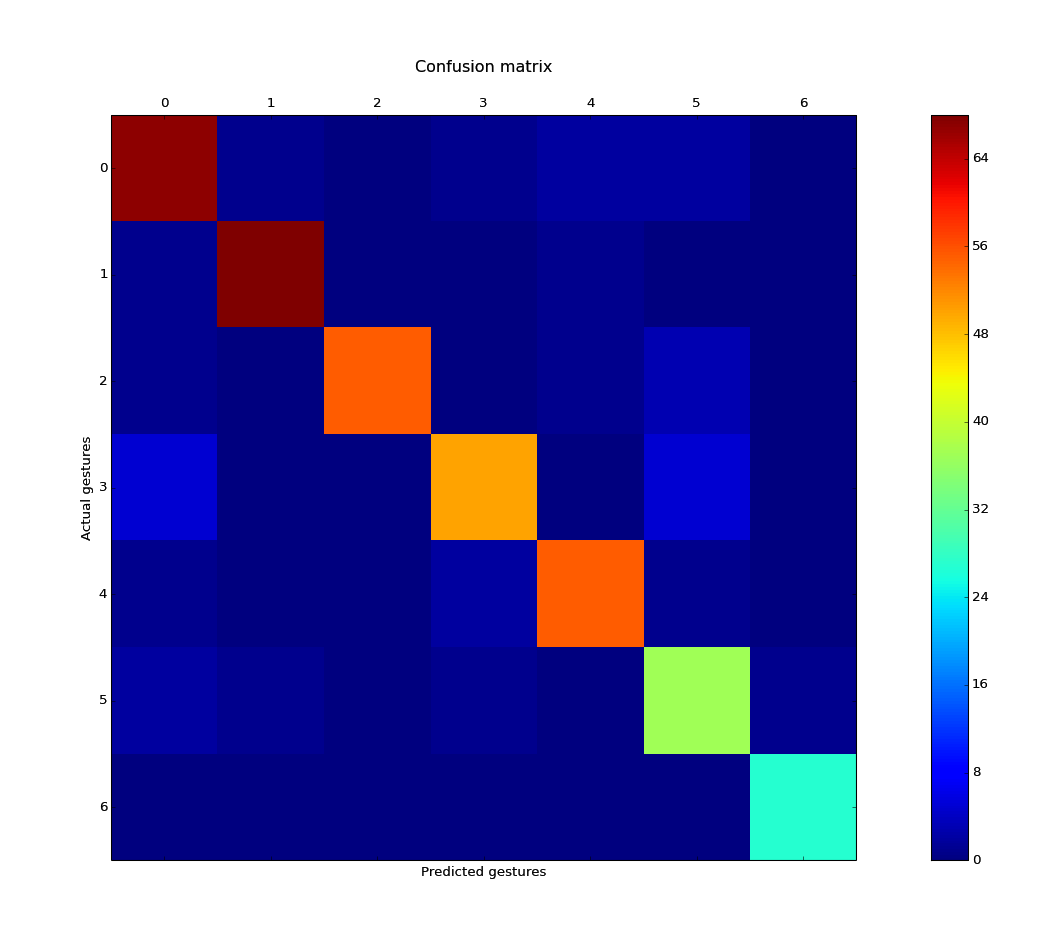
\includegraphics[width=0.3\textwidth]{svm/svm_confusion_matrix.png}
    \caption{Confusion Matrix}
    \label{fig:svm_confusion_matrix}
\end{figure}

\begin{table}[h]
\centering
\begin{tabular}{ccc}
\hline
 \textbf{Gesture} &\textbf{Prec.} & \textbf{Recall} \\
 \hline
  0: \ac{RLO} & 87\% & 92\% \\
 \hline
  1: \ac{TBO} & 97\% & 97\% \\
 \hline
  2: \ac{OT} & 100\% & 92\% \\
 \hline
  3: \ac{SPO} & 93\% & 83\% \\
 \hline
  4: \ac{DPO} & 93\% & 93\% \\
 \hline
  5: \ac{RO} & 77\% & 88\% \\
 \hline
  6: \ac{BNS} \& \ac{BNN} & 96\% & 100\% \\
 \hline
  Average & 92\% & 92\% \\
 \hline
\end{tabular}
\caption[Erkennungsraten einer SVM]{Erkennungsraten einer SVM}
\label{tab:svm_performance}
\end{table}

\subsubsection{Fazit}
Dann fangen wir mal an:

- Training geht relativ flott, so dass unterschiedliche Parameterkombinationen zügig ausprobiert werden können (allerdings sollte man die Standardwerte für die Parameter benutzen, da sie meistens bereits zu guten Ergebnissen führen)
- prinzipiell kann meist eine gute trennende Hyperebene bzw. akzeptable Fehlerrate gefunden werden

- mittels dem Parameter $C$ lässt sich die Margin-Breite der Hyperebene steuern
- je größer dabei $C$ wird, desto kleiner wird der Margin-Wert, desto stärker handelt es sich um ein Overfitting
- ein hoher Wert für den Parameter $gamma$ führt in Kombination mit einem hohen Wert für $C$ zu einem starken Overfitting an die Trainingsdaten
- für sehr kleine Werte von $C$ können sogar Trainigsdaten falsch klassifiziert werden, die linear separierbar sind

- in der Anwendung nehmen wir (bisher) eine relativ große Fehlerrate von 35 Prozent in Kauf, damit wir keinen zu stark an die Trainingsdaten angepassten Klassifikator haben
- da eine Hyperebene, die nicht überangepasst ist, sondern die Klassifikation ''allgemeiner'' mit einigen ''Randunschärfen'' ausführt, wünschenswerter ist

- ''ref/images/svm/svm\_confmat.png'' zeigt die visuelle Repräsentation einer Confusion-Matrix
- dafür wurde das Training der SVM mit etwa 2700 Datensätzen und die Validierung mit etwa 900 Datensätzen durchgeführt
- die durchschnittliche Genauigkeit (Fähigkeit des Klassifikators einen Eingabevektor nicht einer Klasse zuzuordnen, zu der er nicht angehörig ist) liegt bei 67 Prozent
- die durchschnittliche Trefferquote (Fähigkeit des Klassifikators alle entsprechenden Eingabevektoren der richtigen zugehörigen Klasse zuzuordnen) liegt bei etwa 65 Prozent

- persönliche Meinung: ich glaube, die Performance des Klassifikators lässt sich vor allem durch eine bessere Vorverarbeitung und Merkmalsextraktion leicht verbessern.
- allerdings erschweren die unterschiedlich gut aufgenommenen Trainingsdatensätzen von verschiedenen Laptops mit unterschiedlicher Hardwarekonfiguration (Lautsprecher und Mikrofon) die Vorverarbeitungs- und die Trainingsphase und beeinflussen somit stark die Validierungs- und die Live-Klassifikationsergebnisse

- die aktuelle Vorverarbeitungsstrategie erfordert eine recht exakte Ausführung der Geste unter sehr guten Vorraussetzungen, sprich laute Umgebungsgeräusche sollten vermieden werden (dies kann jedoch auch an der aktuellen Hardwarekonfiguration des Laptops liegen), da das Mikrofon überempfindlich reagiert und selbst normale Musik als Umgebungsgeräusche Schwankungen im Frequenzspektrum rund um die Referenzfrequenz von 18.500 kHz verursacht!
